
\documentclass[a4paper, 11pt]{letter}

\usepackage{graphicx}
\usepackage{fancyhdr}
\usepackage{geometry}
\usepackage{indentfirst}
\usepackage[utf8]{inputenc}
\usepackage{color}
\usepackage{colortbl}
\usepackage[dvipsnames]{xcolor}
\usepackage{etoolbox}

\setlength{\textwidth}{18.0cm}
\setlength{\textheight}{28.0cm}
\setlength{\oddsidemargin}{-2.0cm}
\setlength{\evensidemargin}{-2.0cm}
\setlength{\topmargin}{-3.0cm}

\renewcommand{\baselinestretch}{1.2}
% \fontsize{12}{18}\selectfont
\setlength{\parindent}{1.2cm}

\colorlet{lGray}{black!30}
\colorlet{dGray}{black!50}

\def\OptA{Magnetic fusion: turbulence, transport, heating \& confinement}
\def\OptB{Physics \& diagnostics in tokamaks}
\def\OptC{Space plasmas}
\def\OptD{High energu density astrophysical plasmas}
\def\OptE{Low pressure cold plasmas}
\def\OptF{Non-equilibrium plasmas at high pressure}
\def\OptG{Relativistic laser-plasma interaction}
\def\OptH{Laser-plasma interaction and confinement inertial fusion}

\def\SpeA{Diffuse astrophysical plasmas}
\def\SpeB{Numerical simulations \& solar magnetism}
\def\SpeC{Hydrodynamics of inertial fusion}
\def\SpeD{Power \& high energy lasers}
\def\SpeE{Advanced physics for Tokamaks}
\def\SpeF{Tokamaks : experimentation}
\def\SpeG{Plasmas for energy and aerospace applications}
\def\SpeH{Plasmas for materials, environment, biomedicine \& agriculture}

\pagestyle{empty}

\def\Ca{17}
\def\Cb{}
\def\Cc{}
\def\Cd{}
\def\Ce{}
\def\Cf{}
\def\Cg{}

\def\Oa{17}
\def\Ob{}
\def\Oc{}
\def\Od{}
\def\Oe{}
\def\Of{}
\def\Og{}
\def\Oh{}

\def\Sa{}
\def\Sb{}
\def\Sc{}
\def\Sd{}
\def\Se{}
\def\Sf{}
\def\Sg{}
\def\Sh{}

\begin{document}


\includegraphics[height=3.0cm]{su_sciences}

\begin{center}
    Masters of Plasma Physics \& Fusion \\
    Academic year 2023 \\
    Academic transcript \\

    Andrea Ciardi \\
\end{center}

\vspace{1.0cm}

\begin{flushright}
\end{flushright}

\noindent


\begin{tabular}{p{0.6\textwidth}p{0.1\textwidth}p{0.20\textwidth}}
Course Title & Crédit & Score \\
Fisrt semester & & \\
\rowcolor{lGray}
Core & & \\
Tools for plasmas \& fusion                     & 3 & \Ca / 20 \\
Magnetohydrodynamics                            & 3 & \Cb / 20 \\
Kinetic theory \& fusion                        & 3 & \Cc / 20 \\
\arrayrulecolor{dGray}\hline
Waves and instabilities \& fusion               & 3 & \Cd / 20 \\
Numerical methods \& simulations                & 3 & \Ce / 20 \\
Instrumentation, diagnostics \& plasma analysis & 3 & \Cf / 20 \\
Atomic, molecular \& radiation physics          & 3 & \Cg / 20 \\
\arrayrulecolor{dGray}\hline
\rowcolor{lGray}
Options & & \\
\ifdefempty{\Oa}{}{\OptA                        & 3 & \Oa / 20 \\}
\ifdefempty{\Ob}{}{\OptB                        & 3 & \Ob / 20 \\}
\ifdefempty{\Oc}{}{\OptC                        & 3 & \Oc / 20 \\}
\ifdefempty{\Od}{}{\OptD                        & 3 & \Od / 20 \\}
\ifdefempty{\Oe}{}{\OptE                        & 3 & \Oe / 20 \\}
\ifdefempty{\Of}{}{\OptF                        & 3 & \Of / 20 \\}
\ifdefempty{\Og}{}{\OptG                        & 3 & \Og / 20 \\}
\ifdefempty{\Oh}{}{\OptH                        & 3 & \Oh / 20 \\}

\ifdefempty{\Sa}{}{\SpeA                        & 3 & \Sa / 20 \\}
\ifdefempty{\Sb}{}{\SpeB                        & 3 & \Sb / 20 \\}
\ifdefempty{\Sc}{}{\SpeC                        & 3 & \Sc / 20 \\}
\ifdefempty{\Sd}{}{\SpeD                        & 3 & \Sd / 20 \\}
\ifdefempty{\Se}{}{\SpeE                        & 3 & \Se / 20 \\}
\ifdefempty{\Sf}{}{\SpeF                        & 3 & \Sf / 20 \\}
\ifdefempty{\Sg}{}{\SpeG                        & 3 & \Sg / 20 \\}
\ifdefempty{\Sh}{}{\SpeH                        & 3 & \Sh / 20 \\}

\end{tabular}


\medskip


\medskip


\medskip

\begin{center}
\vspace{1.0cm}
\closing{
\fromsig{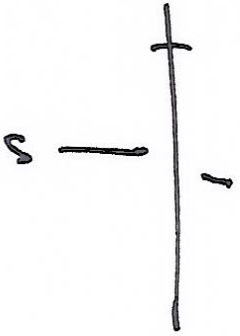
\includegraphics[scale=1]{signature.jpg}} \\
\fromname{Roch SMETS,\\MdC, Sorbonnes Université}
}
\end{center}

\end{document}

